% -*- root: ../../../main.tex -*-
\subsection{Normal Operation | Log Replication}
\label{Log Replication}
Prima di proseguire con la descrizione della seconda fase dell'algoritmo (\textit{log replication}) è bene fornire una definizione completa della struttura del log.
  \subsubsection{Struttura del Log}
  In RAFT ogni server, compreso il leader, mantiene una copia personale del log. Ogni singolo log è strutturato in questo modo:
  \begin{itemize}
    \item{\emph{\textbf{Entry:}}}
    \emph{ogni log è suddiviso in celle chiamate \textbf{entry} identificate da un \textbf{indice} che ne indica la \textbf{posizione} nel log}
    \item{\emph{ogni singola entry si compone di due campi:}}
      \begin{itemize}
        \item{\emph{\textbf{Comando:}}}
        \emph{un comando o una procedura sulla quale tutte le macchine presenti nel cluster devono trovare un accordo.}
        \item{\emph{\textbf{Term:}}}
        \emph{rappresenta il term relativo a quando la entry è stata aggiunta al log. Ciò sta a significare che la entry è stata aggiunta dal leader al suddetto term.}
      \end{itemize}
    \item{\emph{\textbf{Memorizzazione:}}}
    \emph{ogni log è memorizzato in una memoria locale in modo da permettere resistenza ai crash del server.}
    \item{\emph{\textbf{Commited entry:}}}
    \emph{nel momento in cui una entry è replicata sulla maggioranza dei server allora si considera \textbf{committed} e può essere esguita dalle state machine.}
  \end{itemize}
  \begin{figure}[H]
  	\centering
  	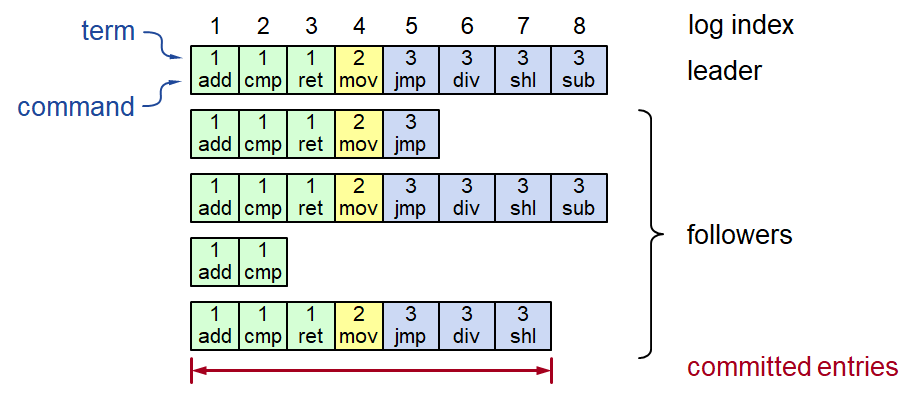
\includegraphics[width=0.99\columnwidth]{raft/logStructure}
  	\caption{Nell'immagine possiamo vedere che la entry n.7 è committed poiché è replicata sulla maggioranza dei server. Entry n.8 non può essere committed poiché è replicata solo su 2/5 dei server.}
  	\label{fig:figure6}
  \end{figure}

  \subsubsection{Log Replication}
  Una volta eletto correttamente, il leader inizia a servire tutte le richieste che provengono dai client. La log replication in situazioni normali procede come segue:
  \begin{enumerate}
    \item{\emph{Il leader \textbf{appende} il comando al proprio log.}}
    \item{\emph{Il leader invia dei messaggi di tipo \textbf{AppendEntries} ai followers.}}
    \item{\emph{Quando la \textbf{maggioranza dei follower} comunica al leader di aver replicato il log allora la entry può essere \textbf{committed}. Nel caso di mancate risposte il leader attende riprovando a inviare la entry.}}
    \item{\emph{Il leader \textbf{passa il comando} alla propria state machine che lo \textbf{esegue}, il \textbf{risultato} viene poi ritornato al client.}}
    \item{\emph{Il leader inoltre comunica ai followers il committment e finalmente li abilita all' esecuzione del comando.}}
  \end{enumerate}
  Il leader mantiene traccia dell'ultima entry che è stata validata e include il suo indice e term in tutte le \textit{AppendEntries} (inclusi gli \textit{heartbeats}). Così facendo i followers potranno rimanere allineati riuscendo quindi ad eseguire in modo tempestivo il comando non appena riconoscono che esso è stato committato.

  \subsubsection{Log Matching Property}
  \label{Log Matching}
  La proprietà di log matching garantisce che:
  \[
    \begin{multlined}
    \emph{\textbf{Se una entry è committed}}\\
    \emph{\textbf{allora anche tutte 
    le entry precedenti lo saranno.}}
    \end{multlined}
  \]
  Questa proprietà deriva da queste sotto-proprietà:
  \begin{itemize}
    \item{\emph{Se due log hanno un entry con lo stesso index e stesso term, allora quell'entry contiene lo stesso comando(sono identiche)}}.
    \item{\emph{Se due \textit{entry} in log diversi hanno lo stesso index e lo stesso term, allora anche tutte le loro precedenti entry sono identiche tra i due log}}.
  \end{itemize}
  La prima proprietà segue dal fatto che un leader può creare \textbf{solamente una entry in un dato index per term} e \textbf{le entry non cambiano mai posizione}.\\
  La seconda proprietà è garantita da un semplice \textbf{consistency check} eseguito dai messaggi \textbf{AppendEntries}.
  \paragraph{Consistency Check e Riparazione del Log}
  \begin{enumerate}
    \item{\textbf{AppendEntries con consistency check:}}
    Nel momento in cui vengono inviate le \textbf{AppendEntries}, il leader include come argomento dei messaggi anche \textbf{l'indice e il term della entry immediatamente precedente la nuova entry da replicare}.
    \[
      AppendEntries(term, index)
    \]
    \item{\textbf{Ack negativo:}}
    Se il follower non trova una entry nel \textbf{fronte del log} con lo \textbf{stesso indice e term} allora rifiuta la nuova entry e manda un \textbf{ack(false)}.
    \[
      Ack(false)
    \]
    \item{\textbf{AppendEntries induttiva:}}
    IL leader allora procede in modo \textbf{induttivo} provando a inviare \textbf{AppendEntries} che fanno riferimento agli indici precedenti. Il leader invia l'\textit{entry} precedente all'ultima inviata; se anch'essa non corrisponde, invia quella ancora prima e così via, fino a trovare una corrispondenza, come in figura \ref{fig:figure8}
    \[
      AppendEntries(term, index - 1)
    \]
    \item{\textbf{Ack positivo:}}
    L'operazione di append ha successo solo nel caso in cui ci sia corrispondenza tra l'elemento precedente del log del leader e l'elemento nella stessa posizione del log del follower. In questo caso viene inviato un messaggio di ack positivo. \textbf{Tutte le entry successive all'indice di match vengono cancellate }
    \[
      Ack(true)
    \]
  \end{enumerate}
  
   
  \begin{figure}[H]
  	\centering
  	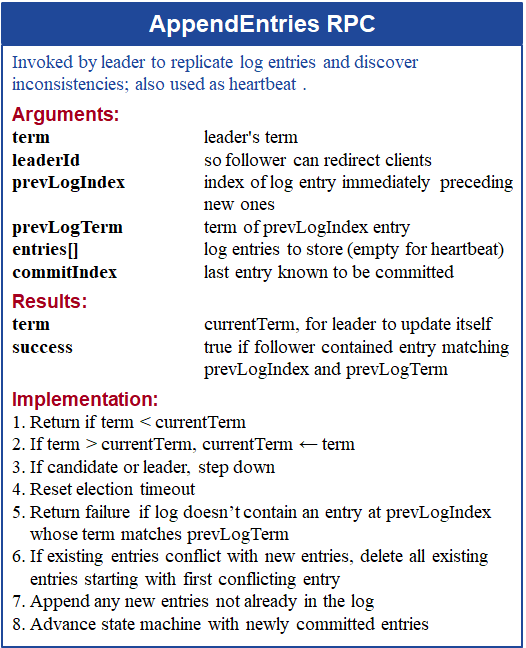
\includegraphics[width=0.99\columnwidth]{raft/appendEntries}
  	\caption{Il leader replica il proprio log inviando un elemento per volta al log dei vari follower, i quali accettano solo se c'è corrispondenza tra l'entry precedente a quella inviata dal leader e la loro ultima entry.}
  	\label{fig:figure7}
  \end{figure}

  \begin{figure}[H]
  	\centering
  	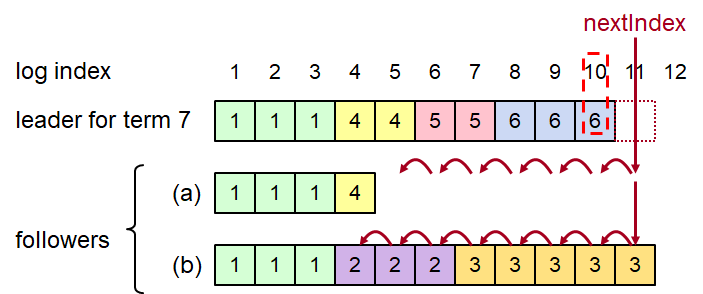
\includegraphics[width=0.99\columnwidth]{raft/repairingFollowerLogs}
    \captionsetup{singlelinecheck=off}
  	\caption[consistencyCheck2]{
    Il leader procede ad inviare entry con \textbf{indice sempre minore} fino a trovare una corrispondenza, per poi risalire fino alla cima del log, se necessario sovrascrive le entry inconsistenti del follower.\\
  	In figura, il leader deve inviare la entry in posizione 10, con term 6.
    \begin{itemize}
      \item{\textbf{Caso a:}}
      L'indice 10 è vuoto, di conseguenza il leader procede a ritroso finché non trova \textbf{corrispondenza} all'indice 4.
      \item{\textbf{Caso b:}}
       All'indice 10 c'è una entry diversa da quella del leader, di conseguenza esso procede a ritroso fino all'indice 3, dal quale inizierà a \textbf{ricostruire il log sovrascrivendo le entry inconsistenti}.
    \end{itemize}
    }
  	\label{fig:figure8}
  \end{figure}
  Il leader continua ad inviare \textit{AppendEntries} ai followers che non rispondono, fino a quando non ottiene successo. Una eventuale presenza minoritaria di follower lenti o bloccati non intacca le performance del cluster e non rallenta la validazione di nuove entry da parte del leader.

  \subsubsection{Crash del Leader e inconsistenze del Log}
  In situazioni normali l'algoritmo garantisce che leader e followers si mantengano consistenti e dunque il \textbf{consistency check} delle \textbf{AppendEntries} non fallisce mai.\\
  Può capitare però che il \textbf{leader crashi prima di riuscire a completare la replica sulla maggioranza dei follower}. In questo caso i log dei follower possono mostrare diversi tipi di inconsistenza (vedi figura \ref{fig:figure9}):
  \begin{itemize}
    \item{Entry mancanti}
    \item{Entry sovrabbondanti}
    \item{Entrambe le situazioni}
  \end{itemize}

  \begin{figure}[H]
    \centering
    \includegraphics[width=0.99\columnwidth]{raft/loginconsistencies}
    \caption[inconsistency]{La figura mostra un esempio in cui vengono mostrati tutti i tipi di inconsistenza possibili in RAFT.}
    \label{fig:figure9}
  \end{figure}
  In RAFT le inconsistenze sono risolte senza introdurre dei comportamenti speciali da parte del leader. Questa semplicità risiede in una importante assunzione che viene fatta dall'algoritmo: \textbf{il leader ha pieno potere e possiede la verità assoluta.}\\
  Questa assunzione permette al leader di portare tutti i server a convergere alla propria visione del log. Questo sta a significare che i follower potrebbero addirittura \textbf{cancellare o riscrivere entry non committate} presenti nei loro log se queste non soddisfano il leader. La riparazione del log viene fatta in modo automatico tramite \textbf{AppendEntries} con \textbf{consistency check induttivo}.